%*----------- SLIDE -------------------------------------------------------------
\begin{frame}[t]{Robôs SCARA} 
    % \begin{figure}
    %     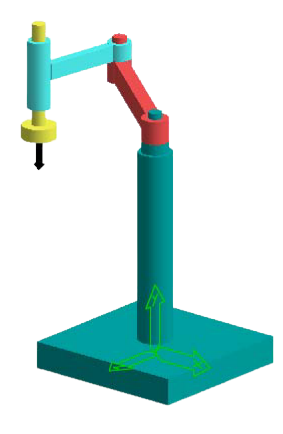
\includegraphics[width=5cm, height=4cm]{scara.png}
    %     %\caption{.}
    % \end{figure}

    \begin{columns}
        % \column{.01\textwidth}
        \column{.01\textwidth}
        \column{.5\textwidth}

        \begin{figure}
            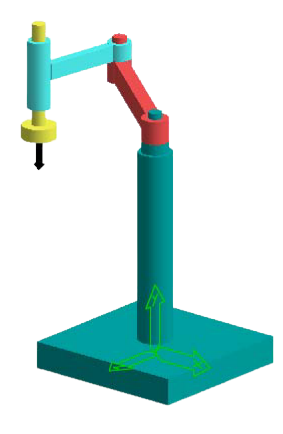
\includegraphics[trim = 0 0 0 0, clip, width=0.5\textwidth]{scara.png}
            %\caption{.}
        \end{figure}

        % \centering
        % $f(n) = \frac{K}{n}$\\
        % $f(n)$ \scriptsize{é a frequência de ocorrência de uma palavra}\\
        % $n$ \scriptsize{é a ordem de frequência}
        % $K$ \scriptsize{é a constante}\\

        \column{.49\textwidth}
        Robôs SCARA ou Selective Compliance Assembly Robot Arm são robôs do tipo
        % A lei de Zipf pontua a frequência com que certas palavras aparecem nos textos científicos de maneira a definir sua representatividade neste contexto.\\
    \end{columns}

    
    % \transdissolve[duration=0.5] % ???
    % A complexidade do conhecimento nas inovações tem aumentado ano após ano. A necessidade do ser humano em alcançar patamares cada vez mais eficientes em nosso dia a dia, faz com que tenhamos cada vez mais uma capacidade de otimização na busca por conhecimento.

    % \centering
    % \vspace*{0.1cm}
    % \Large{O tempo é vital.}

    % \roundpic[xshift=0cm,yshift=0cm]{4cm}{7cm}{time}
    %\newline

        % \begin{columns}[t]
        %     \column{.05\linewidth}
        %     \column{.4\linewidth}
        %         \huge{O tempo é vital.}
        %     \column{.6\linewidth}
        %     \begin{center}
        %     %\centerline{
        %         \begin{figure}
        %             %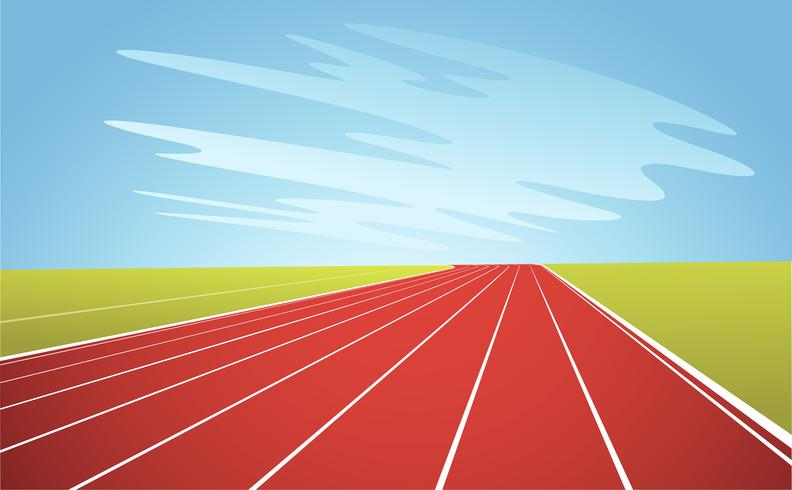
\includegraphics[width=1\textwidth]{pista}
        %             %\caption{Pista de corrida \cite{agostini2007}}
        %             \roundpic[xshift=0cm,yshift=0cm]{4cm}{7cm}{time}
        %             %\caption{Pista de corrida \cite{agostini2007}}
        %         \end{figure}
        %     %}
        %     \end{center}
        % \end{columns}
%*----------- notes
    \note[item]{Notes can help you to remember important information. Turn on the notes option.}
\end{frame}
%-
%*----------- SLIDE -------------------------------------------------------------
\begin{frame}[c]{Modelo Matemático} 
    % \transdissolve[duration=0.5]
    \begin{itemize}
        \item Cinemática
        \item Dinâmica
    \end{itemize}

    % \begin{center}
    %     \Wider{%
    %     \begin{shaded}
    %     \begin{center}
    %         \vspace*{0.5cm}
    %         \resizebox{!}{0.7cm}{%
    %             \textcolor{cyan}{G}\textcolor{red}{o}\textcolor{orange}{o}\textcolor{cyan}{g}\textcolor{teal}{l}\textcolor{red}{e}?
    %         }%
    %     \end{center}
    %     \end{shaded}
    %     }%
    % \end{center}
%*----------- notes
    \note[item]{Notes can help you to remember important information. Turn on the notes option.}
\end{frame}
%-
%*----------- SLIDE -------------------------------------------------------------
\begin{frame}[c]{Cinemática Direta} 
    \framesubtitle{Notação D-H}
    Objetivo: Encontrar pose do end effector a partir dos ângulos e deslocamentos angulares das juntas. \\
    Pela notação D-H é possível descrever uma junta com 4 parâmetros.\\
    % \centering
    % 
\includegraphics[clip, trim = 0 0 0 0,  width=.83\textwidth]{databases.jpg}
%*----------- notes
    \note[item]{Notes can help you to remember important information. Turn on the notes option.}
\end{frame}
%-
%*----------- SLIDE -------------------------------------------------------------
\begin{frame}[c]{Cinemática Inversa} 
    % \framesubtitle{Pouco tempo para muito resultado}
    % \transdissolve[duration=0.5]
    Objetivo: Encontrar ângulos e deslocamento angulares das juntas a partir da pose do end effector.
    % \centering
    % 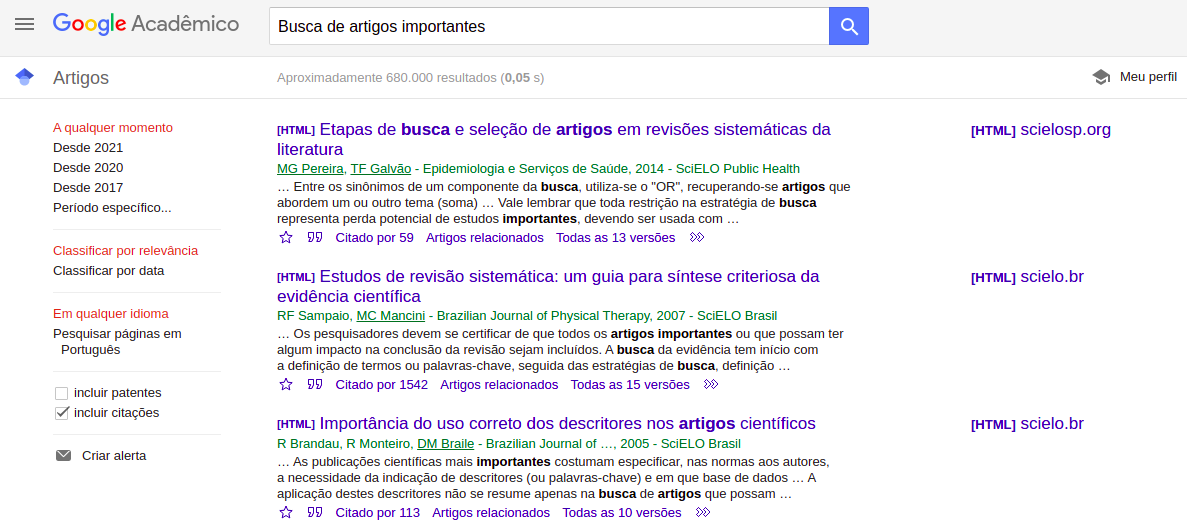
\includegraphics[clip, trim = 0 0 0 0,  width=1\textwidth]{googleacademico2.png}
%*----------- notes
    \note[item]{Notes can help you to remember important information. Turn on the notes option.}
\end{frame}
%-
%*----------- SLIDE -------------------------------------------------------------
\begin{frame}[c]{Como vocês realizam as buscas por artigos?} 
    \framesubtitle{Pouco tempo para muito resultado}
    \transdissolve[duration=0.5]
   
    \centering
    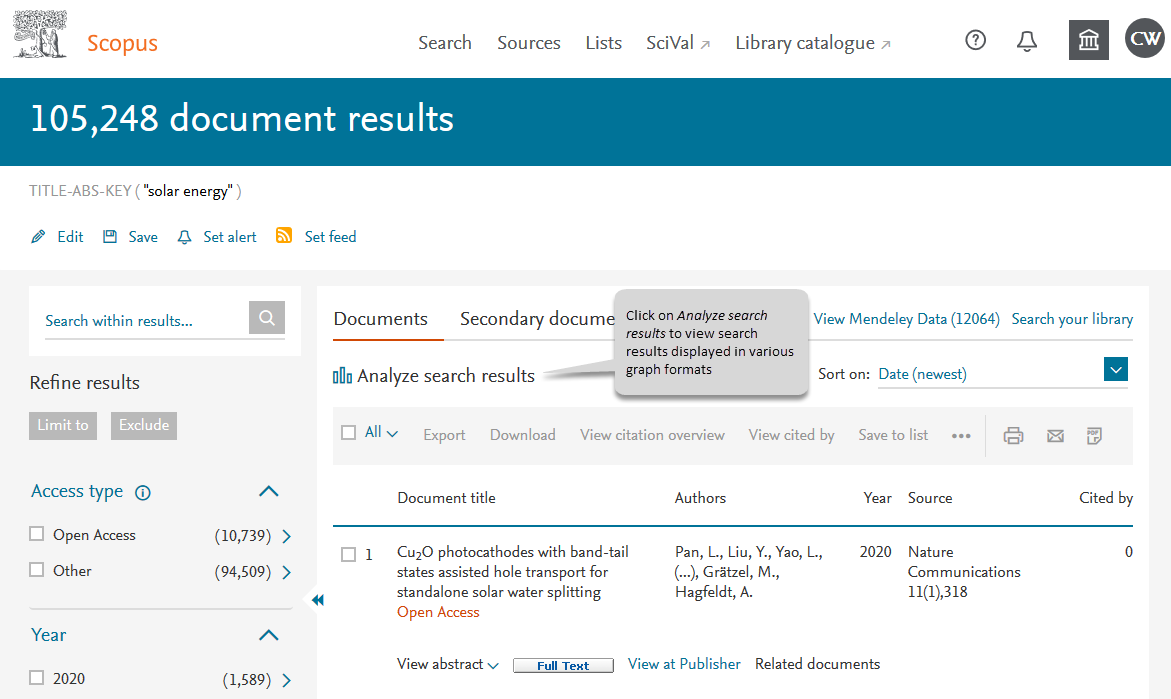
\includegraphics[clip, trim = 0 0 0 0,  width=.75\textwidth]{scopus.png}
%*----------- notes
    \note[item]{Notes can help you to remember important information. Turn on the notes option.}
\end{frame}
%-
%*----------- SLIDE -------------------------------------------------------------
\begin{frame}[c]{Modelo matemático} 
    \framesubtitle{Pouco tempo para muito resultado}
    \transdissolve[duration=0.5]
   
    \centering
    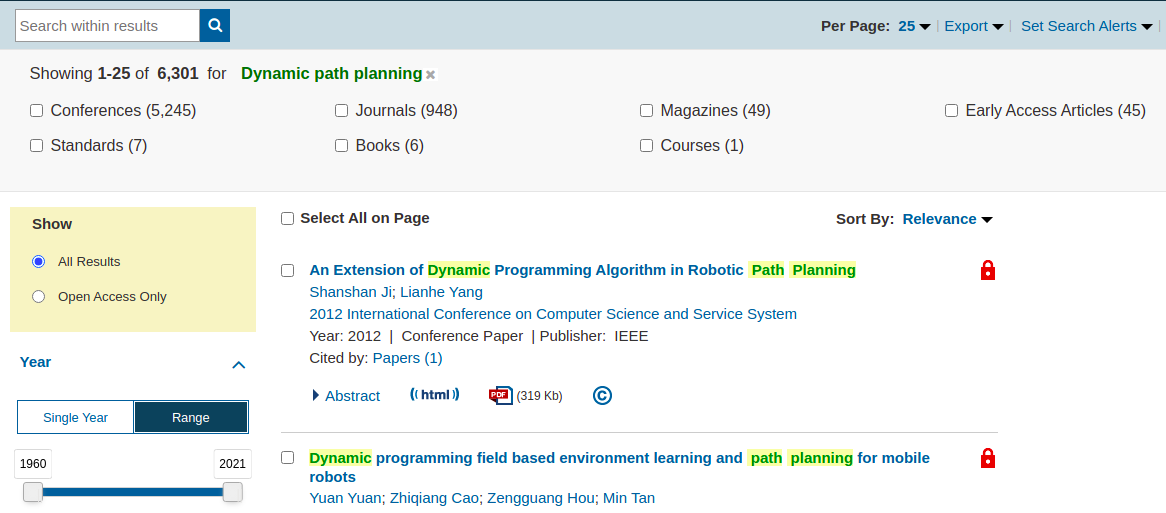
\includegraphics[clip, trim = 0 0 0 0,  width=1\textwidth]{ieee.png}
%*----------- notes
    \note[item]{Notes can help you to remember important information. Turn on the notes option.}
\end{frame}
%-
%*----------- SLIDE -------------------------------------------------------------
\begin{frame}[t]{Tempo e precisão}
    \transboxout[duration=0.5]
    %\framesubtitle{Darwin-OP}
    Uma das vertentes da tecnologia é a capacidade de tornar os processos mais rápidos e precisos, suportando a vida humana no planeta.

    \vspace*{0.2cm}
    Alguns fatores impulsionadores
		\begin{itemize}
			\item Competitividade
			\item Prazo de entrega
			\item Concluir um trabalho 
		\end{itemize}

    \vspace*{0.2cm}
    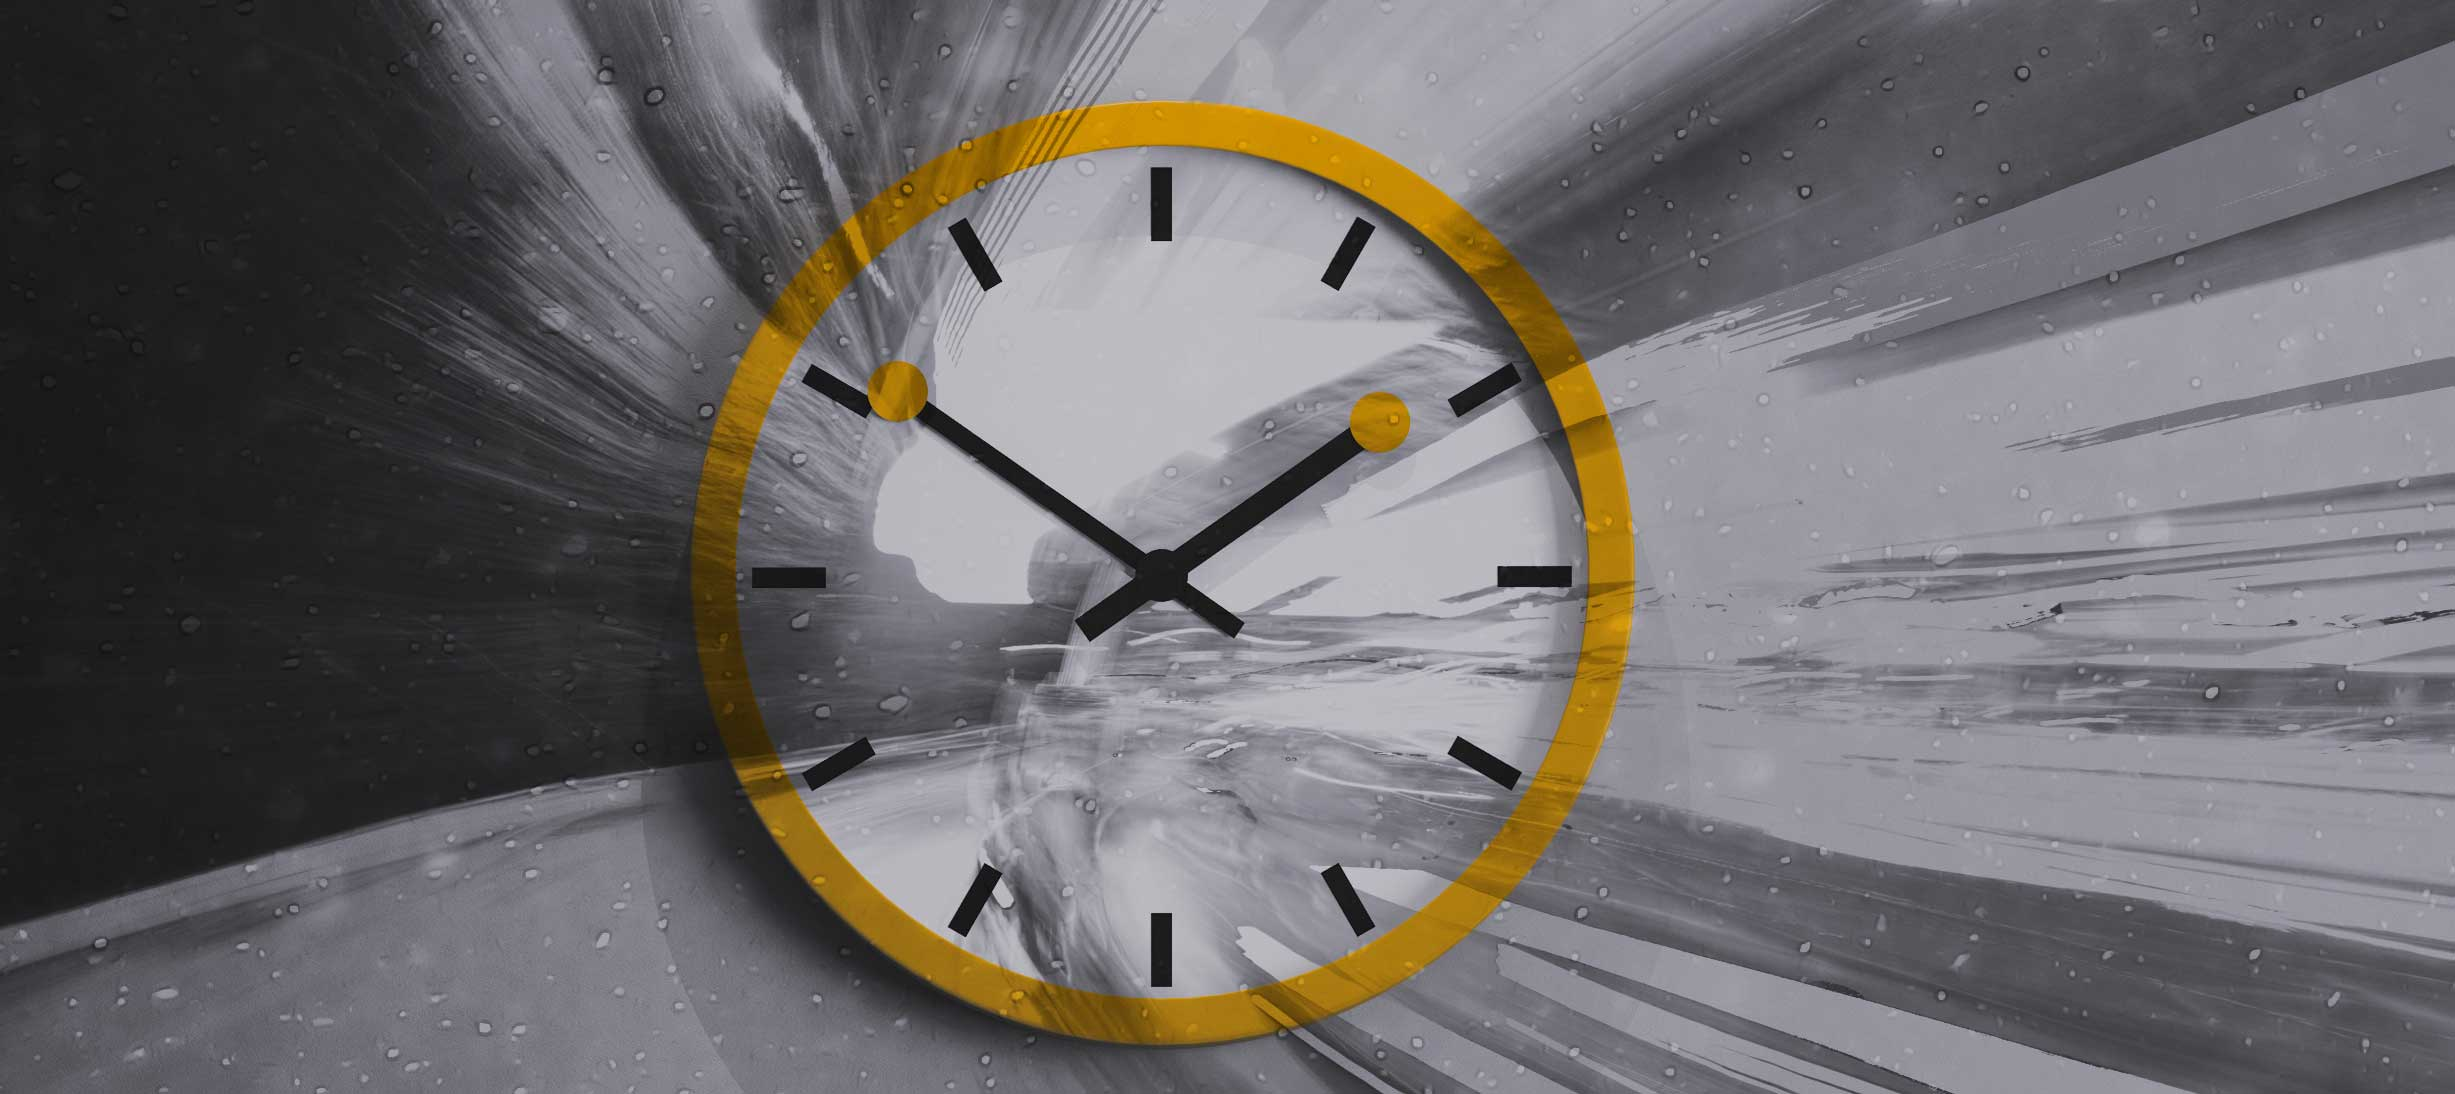
\includegraphics[clip, trim = 0 420 0 80, width=1\textwidth]{time-and-precision.jpeg}

    \begin{columns}
        \column{.1\textwidth}
        \column{.5\textwidth}
        \column{.4\textwidth}
    \end{columns}
%*----------- notes
    \note[item]{Notes can help you to remember important information. Turn on the notes option.}
\end{frame}
%-
